\section{\label{sec:YSO}{Rare earth doped Y$_{2}$SiO$_{5}$}}

\subsection{YSO Crystal Structure}
Yttrium Orthosilicate is a monoclinic crystal with with Si$^{4+}$ tetrahedral and lanthanide Y$^{3+}$ octahedral site symmetry \citep{SHOUDU1999901}. The Czochralski-growth technique for rare earth orthosilicates is detailed in Ref.~\citep{MELCHER19931001}. Depending on the growth temperature there are two possible monoclinic crystal structures which can form (X1 or X2). The Y$^{+3}$ ions can be substituted by activator rare earth ions. There are two inequivalent Y$^{+3}$ atomic sites with low C1 point symmetry for either crystal phase commonly referred to as site I and site II \citep{doi:10.1021/jp5050207}. The sites have a different volume due to the proximity of oxygen atoms. Therefore RE ions with radii larger than the Y$^{3+}$ radii (0.892 $\AA$) preferentially occupy the site I~\citep{nikl2016nanocomposite}.     

\begin{figure}[h]
\centering
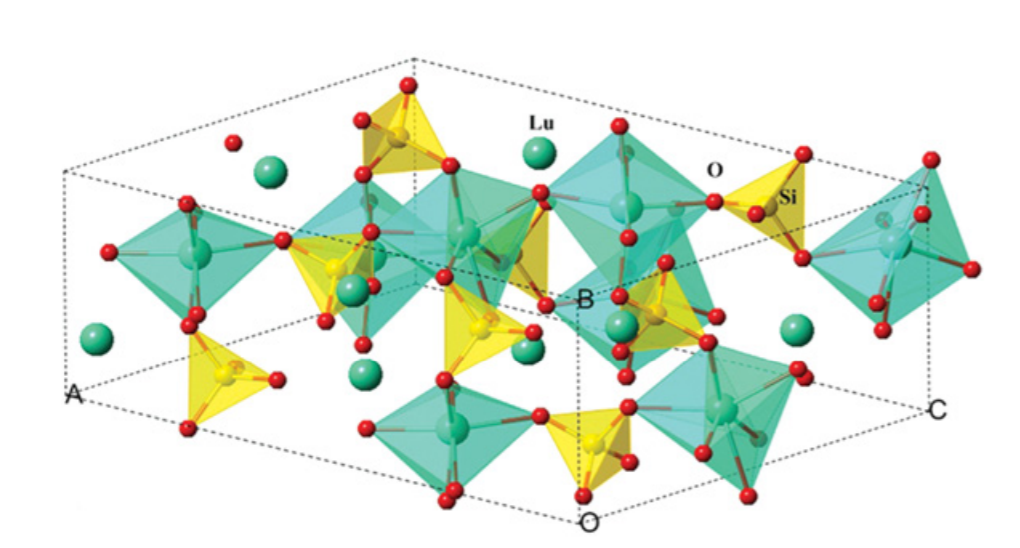
\includegraphics[height=0.32\textwidth,keepaspectratio]{YSOstructure}
\caption{\label{fig:YSOstructure} RE$_{2}$SiO$5$ crystal structure \citep{Ceramics}.}
\end{figure}


The space group of YSO is C$^{6}_{2h}$ with two-fold symmetry of the crystallographic $b$ axis (see Section.~\ref{sec: YSO stiffness matrix}). Therefore each site has two sub-sites which are related through 180$^{\circ}$ crystal rotation. The sub-sites are equivalent only when an applied magnetic field is parallel or perpendicular to the b-axis~\citep{PhysRevB.97.064409}. In addition to the nonorthogonal crystallographic axes, a monoclinic biaxial crystal has a set of orthogonal dielectric axes ($D1,D2,D3$) due to the three principle refractive indices. The b-axis is parallel to the $D3$-axis. The $D1$ and $D2$ axis are measured by placing the crystal between a crossed polarizer and applying a laser parallel to the $b$-axis. Rotation of the crystal perpendicular to the laser identifies the dielectric axes as no light is transmitted when $D1$ or $D2$ are collinear to the polarizers \citep{Traum:14}.     

%Therefore, the crystal is cut along the dielectric frame (D1,D2,b).

 
\subsection{Electronic Structure of Rare-earth Ions}


Rare earth elements are a group containing lanthenides, Scandium and Yttrium. In the 1950's P.P. Feofilov was one of the first physicists to investigate the optical spectroscopy of rare-earth activated crystals for applications in quantum electronics~\citep{MALKIN198713}. He observed diverse spectra dependent on the preparation method of the host material. The name rare earths is a misnomer as they are actually rather abundant in the Earth's core. However, the issue is extracting RE ions as mining of a single element is not possible. These elements exist in ores contain many different metals, with extremely similar chemical properties~\citep{benelli2015introduction}.  
   

\begin{figure}[h]
\centering
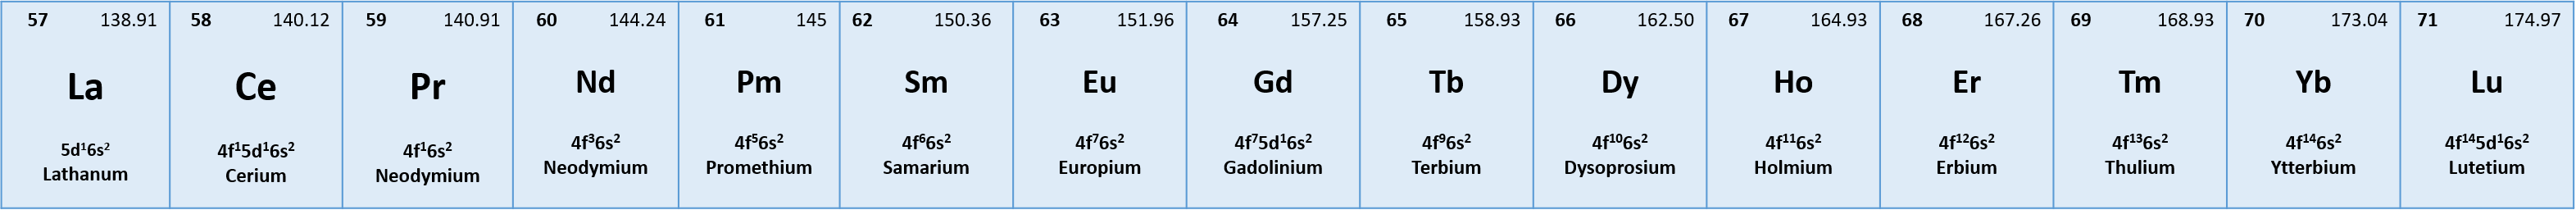
\includegraphics[height=0.08\textwidth,keepaspectratio]{rarearthelements}
\caption{\label{fig:YSOstructure}Lanthanide group elements with electron configuration beginning with [Xe].}
\end{figure}


Rare-earth ions may have an partially filled 4f$^{m}$ ($1 < m < 13$) electron shell, whilst the outer $n = 5$ and $n = 6$ shells are filled. Therefore the paramagnetic center experiences a shielding effect from the environment by the distribution of electrons of the $n = 5$ and $n = 6$ shells. The electronic energy levels of an RE ion can be solved using the central field approximation where each electron moves independently but experiences a nuclear field and an spherically averaged central field due the interaction with other electrons \citep{liu2006spectroscopic}. For a $N$-electron RE ion is given as:

\begin{equation}
\label{eq:freeionHamiltonian}
\hat{H}_{N-el} = \hat{H}_{0} + \hat{H}_{el-el} + \hat{H}_{spin-orbit},
\end{equation} 

\noindent where the dominant $\hat{H}_{0}$ describes the kinetic and potential energy of the electrons in the nuclear field, where $r_{i}$ is the radial distance of electron $i$: 

\begin{equation}
\label{eq:H0}
\hat{H}_{0} = -\sum{N}{i=1} \frac{\hbar^{2}}{2m} \nabla_{i}^{2} - \sum{N}{i=1}\frac{Ze^{2}}/r_{i}. 
\end{equation} 

\noindent The electron-electron Coulomb repulsion is captured by $\hat{H}_{el-el}$:

\begin{equation}
\label{eq:coloumbrep}
\hat{H}_{el-el} = \sum{N}{i<j} \frac{e^{2}}{r_{ij}},
\end{equation}

\noindent where $r_{ij}$ is the distance between pairs of electrons. The fine structure splitting arises due to the interaction of $\mu_{e}$ with the orbital field: 


\begin{equation}
\label{eq:spinorbit}
\hat{H}_{spin-orbit} = \sum{N}{i} \xi(r_{i})\hat{\bm{L}} \cdot \hat{\bm{S}},
\end{equation}

\noindent where $\hat{\bm{L}}$ is the orbital angular momentum operator and $\xi(r_{i})$ is the spin-orbital coupling constant which is a function of $\xi(r_{i})$. This lifts the degeneracy of $^{(2s+1)}L_{j}$ multiplets where the total angular momentum $\bm{j} = \bm{s} + \bm{l}$. 

\begin{table}[h]
 \begin{center}
  \caption{Energy level scales of RE ions}
  \label{tab:REionenergyscale}
  \begin{tabular}{l | c}
  \hline
  Interaction Mechanism & Energy (cm$^{-1}$)\\
  \hline
  Coulomb repulsion & 10$^{4}$\\
  Spin orbit coupling & 10$^{3}$\\
  Crystal field interaction & 10$^{2}$\\
  Hyperfine splitting & 10$^{-3}$-10$^{-1}$\\
  
  \hline
    \end{tabular}
  \end{center}
\end{table}

When ions are placed in a crystal expectation the crystal field produces the dominant Hamiltonian term. However, due to the shielding of the 4f shell the unpaired electrons remain localised to the nucleus and only interact weakly with the ligands~\citep{MALKIN1987131}. The scale of crystal field splitting compared to other energy splitting of other interaction terms is given in Table~\ref{tab:REionenergyscale}. Therefore the crystal field interaction is treated as a perturbation which produces a Stark shift of the multiplets. Additionally the crystal field distorts the electronic orbitals resulting in the highly magnetic anisotropy of RE doped YSO~\citep{abragam2012electron,KOLMAKOVA1996245}. Further splitting of the fine structure occurs due to the electron Zeeman, hyperfine and nuclear Zeeman interaction detailed in Section ~\ref{sec:zeeman} and ~\ref{sec:hyperfine}. The additional, Zero-field interaction and nuclear quadrupole interaction, spin Hamiltonian terms must be included when $S >\frac{1}{2}$ and $I > \frac{1}{2}$, respectively.      

\subsection{\label{sec:YSOdopedYbions}YSO doped with Yb$^{3+}$ ions}
The stable oxidation $+2$ state of Yb is shown in Fig.~\ref{fig:YSOstructure}. However, Yb$^{3+}$ ions have attractive properties due to their 4f$^{13}$ configuration. Yb$^{3+}$ is a paramagnetic rare earth comprising of two energy levels, the ground $^{2}$F$_{5/2}$ and excited $^{2}$F$_{7/2}$ state \citep{PhysRevB.94.155116}. Additionally, the $I \neq 0$ naturally occurring isotopes are $^{171}$Yb$^{3+}$ ($I=\frac{1}{2}$) and $^{173}$Yb$^{3+}$ ($I=\frac{5}{2}$). Therefore, $^{171}$Yb$^{3+}$ doped in YSO provides the simplest RE hyperfine energy structure which can be investigated using pulsed EPR techniques.  

Yb$^{3+}$ ions with a radii of 0.858 $\AA$ substitute Y$^{3+}$ ions in site I and site II approximately equally. The $\bm{g}$ and $\bm{A}$ tensors for Yb$^{3+}$:YSO have be experimentally extracted in Ref.~\citep{PhysRevB.94.155116}. The site I and site II ground $^{2}$F$_{7/2}$ state dimensionless g-tensors are given below as:

 
\begin{equation}
\label{eq:gtensorsiteI}
\bm{g}_{siteI}=\begin{bmatrix}
3.19 & -0.91 & 0.31 \\ 
-0.19 & -0.54 & 0.15\\ 
0.31 & 0.15 & 1.00 \\
\end{bmatrix}_{(D1,D2,b)},
\end{equation}  
  


\begin{equation}
\label{eq:gtensorsite}
\bm{g}_{siteII}=\begin{bmatrix}
-0.32 & -0.86 & -1.21 \\ 
-0.86 & -0.05 & 1.10 \\ 
-1.21 & 1.10 & -2.57 \\
\end{bmatrix}_{(D1,D2,b)}.
\end{equation}  


Additionally the ground state anisotropic $\bm{A}$ tensors (in MHz) for site I and site II are given below as:


\begin{equation}
\label{eq:AtensorsiteI}
\bm{A}_{siteI}=\begin{bmatrix}
-3844 & 1356 & 1909 \\ 
1356 & -2257 & 162 \\ 
1909 & 162 & -1340 \\
\end{bmatrix}_{(D1,D2,b)},
\end{equation}  

\begin{equation}
\label{eq:AtensorsiteII}
\bm{A}_{siteI}=\begin{bmatrix}
1054 & -503 & -894 \\ 
-503 & 232 & 660\\ 
-894 & 660 & -4554 \\
\end{bmatrix}_{(D1,D2,b)}.
\end{equation}  

The spin relaxation time $T_{1}$ of unpaired electrons spins of Yb$^{3+}$ is highly temperature dependent. This is due to spin coupling to vibrations of the host lattice. For very low temperature (<4 K) the direct process dominates. The rate of the direct process for the case where $k_{B}T$ is greater than the Zeeman splitting is:

\begin{equation}
\label{eq:coloumbrep}
R_{dp} \approx \frac{2\alpha_{D}(\theta)k_{B} T g^{2}_{eff} B^{4}}{\mu},
\end{equation}

\noindent where the constant $\alpha_{D}(\theta)$ varies with crystal orientation as determined in Ref.~\citep{PhysRevB.97.064409}. This process results in direct phonon absorption from the lattice or phonon emission. 


\begin{figure}[h]
\centering
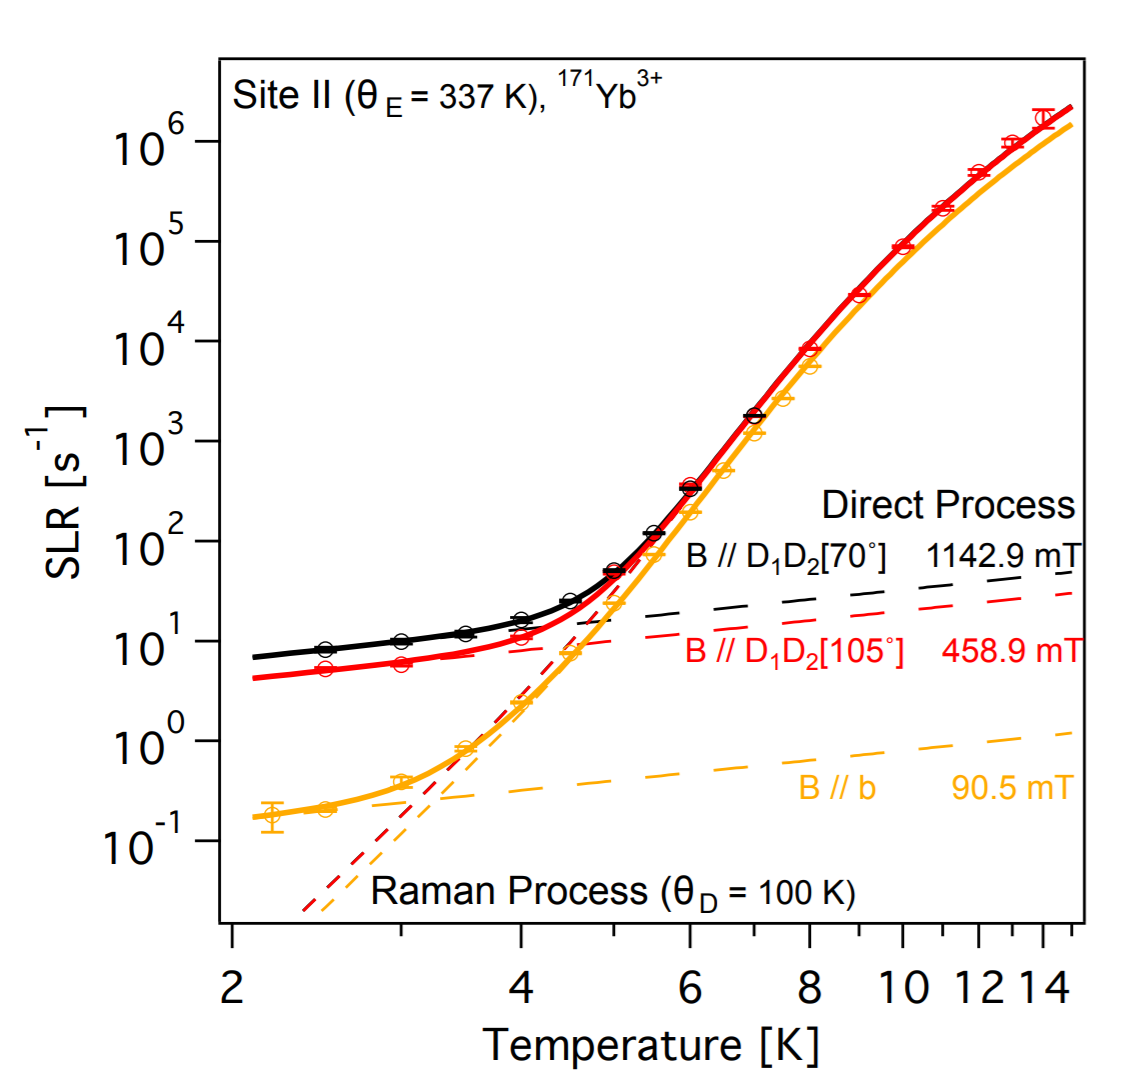
\includegraphics[height=0.4\textwidth,keepaspectratio]{spinrelaxationtime}
\caption{\label{fig:spinrelaxation}Spin relaxation of $^{171}$Yb$^{3+}$:YSO measurements for Site II. Each colour represents a different orientation of crystal with respect to an applied magnetic field. The solid lines are the fit based on a model including both the direct and two-phonon processes. The large dashed line illustrate is the single phonon fit model and the smaller dashed line represents the two-phonon process fit model \citep{PhysRevB.97.064409}.}
\end{figure}

As temperature increases two phonon process become dominant. The Raman process occurs where there is a virtual transition of the spin state to an intermediate state due to the absorption of a phonon. This is followed by emission of phonon with a higher energy due to the transition to the lower spin state. The spin relaxation times has a dependence on temperature which can vary between $T^{-5}-T^{-9}$.Additionally the Orbach process describes the resonant excitation of phonons to a highly excited states which has a temperature dependence of $exp{-\Delta/k_{B}T}$ where $\Delta$ is the excitation energy \citep{weil1994electron,doi:10.1002/pssb.2221170202}.

   



